Container types were a primary motivation for the introduction of templates into the C++ programming language. Prior to templates, polymorphic hierarchies were a popular approach to containers. A popular example was the National Institutes of Health Class Library (NIHCL), which to a large extent translated the container class hierarchy of Smalltalk (see Figure 18.5).

\begin{center}
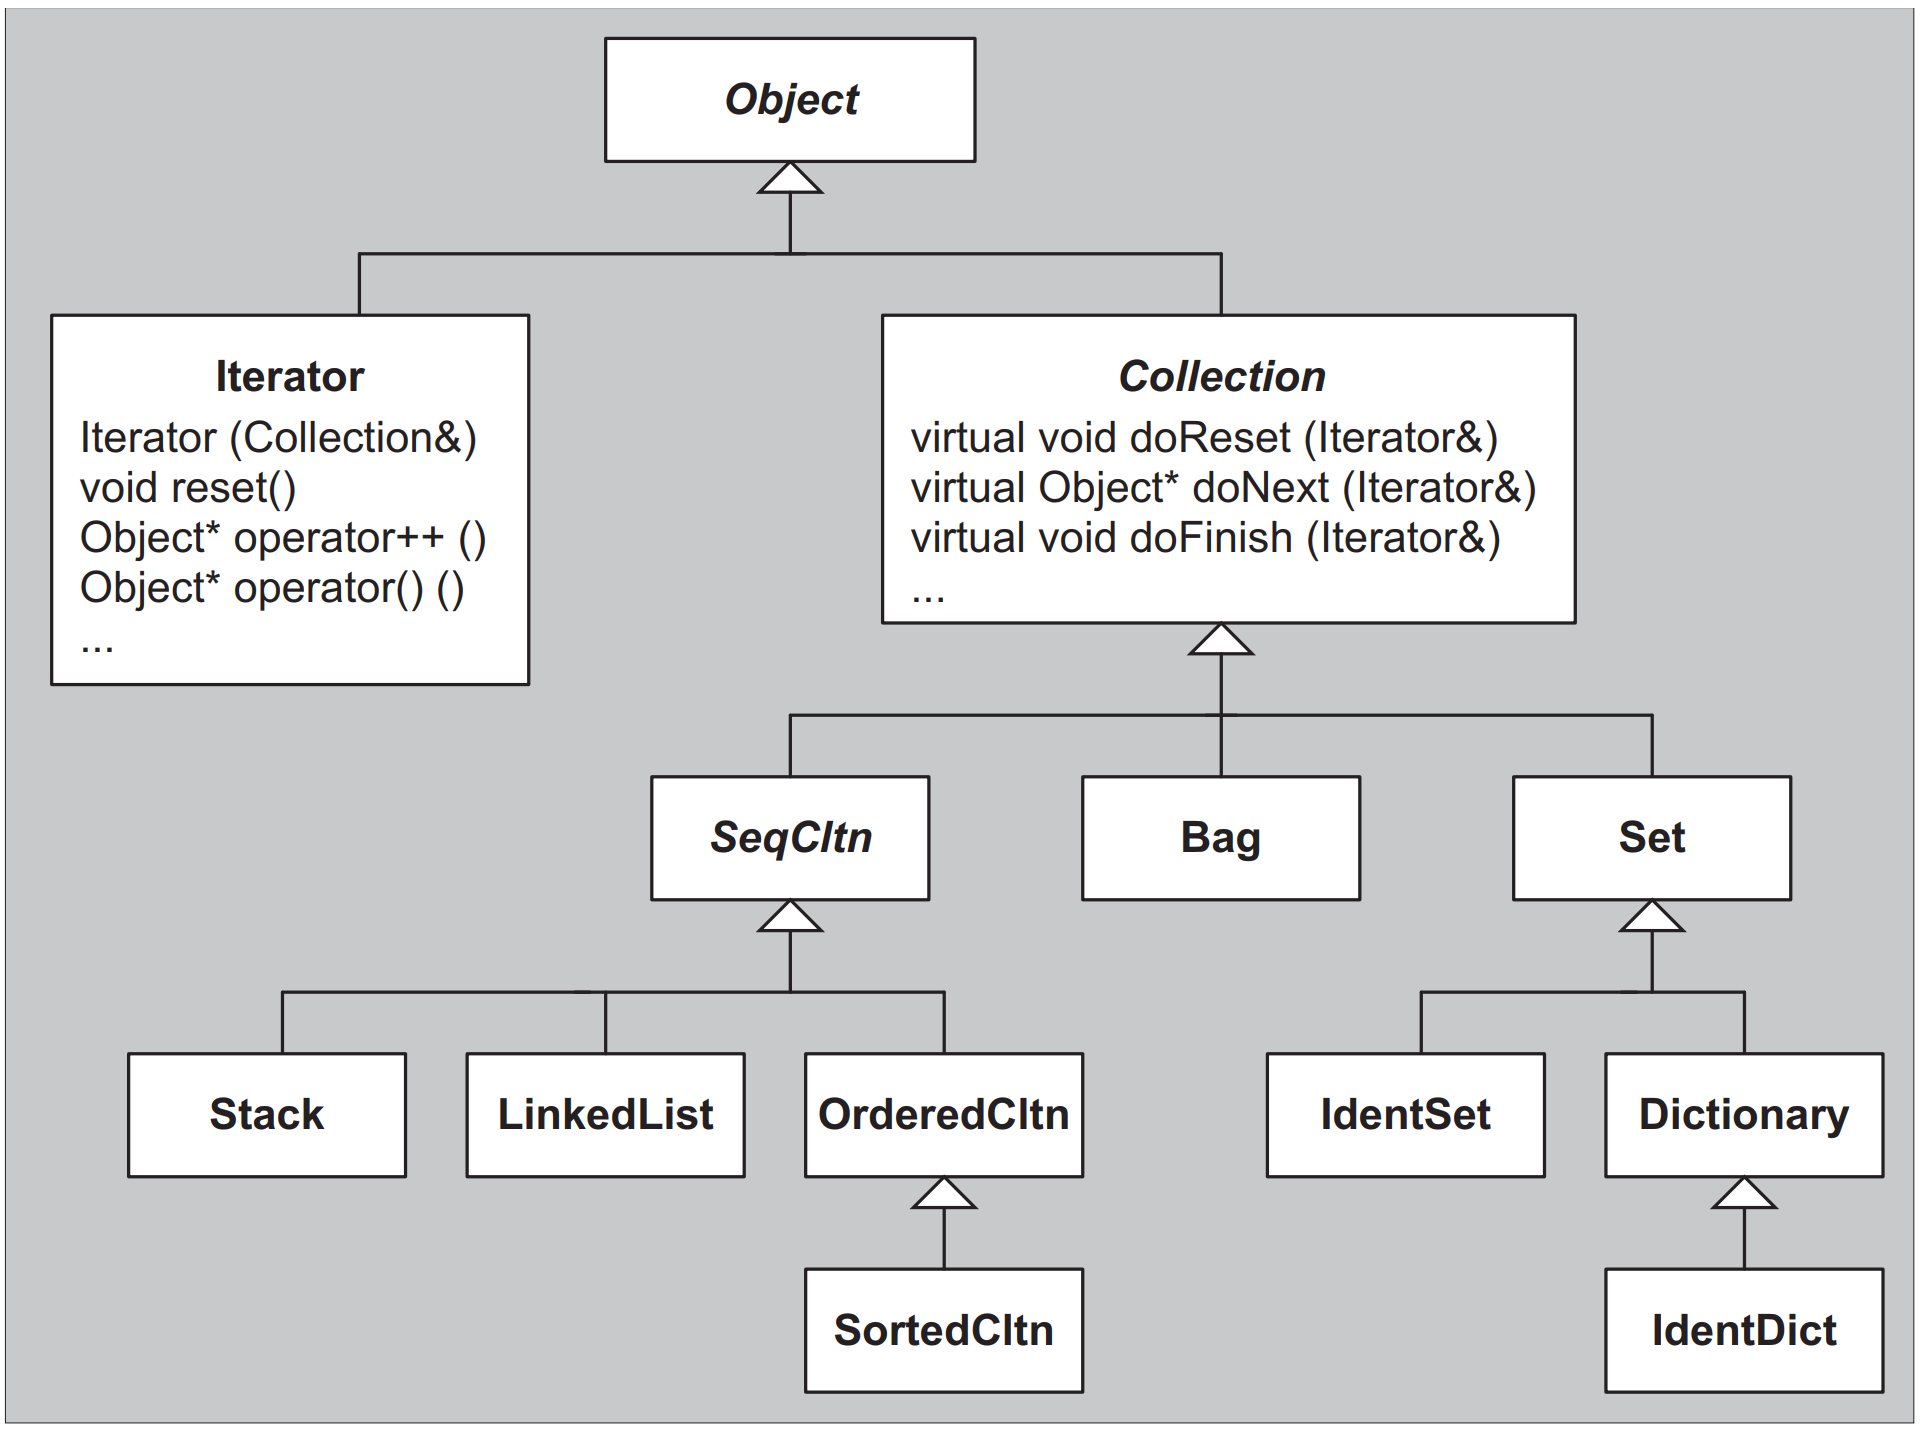
\includegraphics[width=0.8\textwidth]{content/3/chapter18/images/5.png} \\
Figure 18.5. Class hierarchy of the NIHCL
\end{center}

Much like the C++ standard library, the NIHCL supported a rich variety of containers as well as iterators. However, the implementation followed the Smalltalk style of dynamic polymorphism: Iterators used the abstract base class Collection to operate on different types of collections:

\begin{lstlisting}[style=styleCXX]
Bag c1;
Set c2;
...
Iterator i1(c1);
Iterator i2(c2);
...
\end{lstlisting}

Unfortunately, the price of this approach was high in terms of both running time and memory usage. Running time was typically orders of magnitude worse than equivalent code using the C++ standard library because most operations ended up requiring a virtual call (whereas in the C++ standard library, many operations are inlined, and no virtual functions are involved in iterator and container interfaces). Furthermore, because (unlike Smalltalk) the interfaces were bounded, built-in types had o be wrapped in larger polymorphic classes (such wrappers were provided by the NIHCL), which in turn could lead to dramatic increases in storage requirements.

Even in today’s age of templates, many projects still make suboptimal choices in their approach to polymorphism. Clearly, there are many situations in which dynamic polymorphism is the right choice. Heterogeneous iterations are an example. However, in the same vein, many programming tasks are naturally and efficiently solved using templates, and homogeneous containers are an example of this.

Static polymorphism lends itself well to code fundamental computing structures. In contrast, the need to choose a common base type implies that a dynamic polymorphic library will normally have to make domain-specific choices. It’s no surprise then that the STL part of the C++ standard library never included polymorphic containers, but it contains a rich set of containers and iterators that use static polymorphism (as demonstrated in Section 18.6 on page 380).

Medium and large C++ programs typically need to handle both kinds of polymorphism discussed in this chapter. In some situations, it may even be necessary to combine them very intimately. In many cases, the optimal design choices are clear in light of our discussion, but spending some time thinking about long-term, potential evolutions almost always pays off.





















